\section{Measuring Discursive Sophistication}

\subsection{Item Wording}
\begin{frame}{Factual Knowledge Questions}
\begin{itemize}
\item \emph{\cite{carpini1993measuring}}: House majority, veto override percent, party ideological location, judicial review, identifying the vice president
\item \emph{2012 ANES}: Number of times president can be elected, size of federal deficit, full term of senator, meaning of medicare, federal government spending
\item \emph{2015 YouGov}: Speaker of the House, TTIP, Chair of Federal Reserve Board, unemployment rate, veto override percent, common core, largest electricity source, Senate majority
\end{itemize}
\end{frame}
% Carpini: 780 citations

\begin{frame}{Open-Ended Items: 2012 ANES}
\begin{itemize}
\item Is there anything in particular about [CANDIDATE] that might make you want to vote for him? [...] What is that?
\item Is there anything in particular about [CANDIDATE] that might make you want to vote against him? [...] What is that?
\item Is there anything in particular that you like about [PARTY]? [...] What is that?
\item Is there anything in particular that you don't like about [PARTY]? [...] What is that?
\end{itemize}
\end{frame}

\begin{frame}{Open-Ended Items: 2015 YouGov}
\begin{itemize}
\item Do you favor or oppose stricter gun control laws? [...] Still thinking about the question you just answered, what thoughts came to mind while you were answering that question? Please try to list everything that came to mind.
\item Thinking about the mass shootings that have occurred in the U.S. in the last few years, what factors do you think are responsible for the shootings?
\item Do you support or oppose the health care law passed by the President and Congress in 2010?
[...] Still thinking about the question you just answered, what thoughts came to mind while you were answering that question? Please try to list everything that came to mind.
\item For decades, experts have observed that the United States spends far more per person on health care than any other country. However, the U.S. falls behind on most measures of health care outcomes, such as life expectancy. What factors do you think are responsible for the state of our health care system?
\end{itemize}
\end{frame}

\begin{frame}{Open-Ended Items: 2008--2012 Swiss Referenda}
\begin{itemize}
\item Which are your main reasons for accepting/rejecting the proposal [X]?
\item What are additional reasons for accepting/rejecting the proposal [X]?
\end{itemize}
\end{frame}

\subsection{Opinionation}
\begin{frame}{\hyperlink{components}{Opinionation}}\label{opinionation}\centering
\emph{Opinionation$_i$} = $\dfrac{-\sum_{j=1}^J p_{ij} \ln p_{ij}}{\ln J}$
\vspace{1em}\\
\begin{tabular}{lp{9cm}}
	\toprule
	$i$ & Respondent \\
	$j \in \{1,...,J\}$ & Open-ended items \\
	$p_{ij}$ & Proportion of words in the response of individual $i$ to question $j$ relative to the overall size of the individual's response\\
\end{tabular}
\end{frame}

\subsection{Considerations}
\begin{frame}{\hyperlink{components}{Considerations}}\label{elaboration}\centering
\emph{Considerations}$_i$ = $\dfrac{|\mathcal{T}^*_i|}{\max|\mathcal{T}^*_i|}$
\vspace{1em}\\
\begin{tabular}{lp{8.5cm}}
\toprule
$i$ & Respondent \\
$\mathcal{T}^*_i $ & Topic representation of response set $\mathcal{W}_i$, such that $w\rightarrow t^*\forall w \in \mathcal{W}_i$ \\
$w \in \mathcal{W}_i$ & Individual word $w$ in response set $\mathcal{W}_i$\\

$t^* \in \{1,...,T\} $ & Topic $t^*$ out of total number of topics $T$ assigned to $w$ such that $P(t^*|w,X_i) > P(t|w,X_i) \forall t\neq t^*$\\
& $P(t|w,X_i)=\dfrac{P(w|t)P(t|X_i)}{P(w|X_i)}$ \\
$X_i$ & Covariates used in structural topic model
\end{tabular}
\end{frame}

\subsection{Word Choice}
\begin{frame}{\hyperlink{components}{Word Choice}}\label{eloquence}\centering
\emph{Word Choice$_i$} = $\dfrac{\log\sum_{\mathcal{W}_i} P(w|t^*)}{\max\left[\log\sum_{\mathcal{W}_i} P(w|t^*)\right]}$
% estimated max topic probabilities of terms
\vspace{1em}\\
\begin{tabular}{lp{8.5cm}}
\toprule
$i$ & Respondent \\
$w \in \mathcal{W}_i$ & Individual word $w$ in response set $\mathcal{W}_i$\\
%$P(w|t^*)$ & Probability of word $w$ for assigned topic $t^*$ \\
$t^* \in \{1,...,T\} $ & Topic $t^*$ out of total number of topics $T$ assigned to $w$ such that $P(t^*|w,X_i) > P(t|w,X_i) \forall t\neq t^*$\\
& $P(t|w,X_i)=\dfrac{P(w|t)P(t|X_i)}{P(w|X_i)}$ \\
%&$P(t|w,X_i)=\dfrac{P(w|t)P(t|X_i)}{\sum_{j=1}^{T}P(w|t_j,X_i)P(t_j|X_i)}$ \\
$X_i$ & Covariates used in structural topic model
\end{tabular}
\end{frame}
% Is a respondent using high probability terms for each topic?



\subsection{}
\begin{frame} %[allowframebreaks]
\frametitle{\hyperlink{corplot_components}{Comparison with Conventional Measures -- 2012 ANES}}\label{corplot}
  \begin{figure}
  %\only<1>{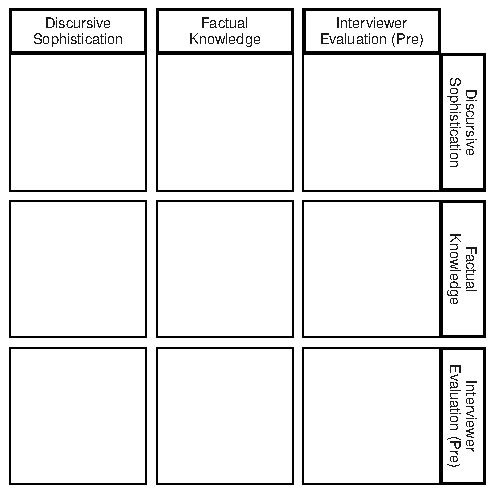
\includegraphics[height=.85\textheight]{fig/corplot_empty.pdf}}
  \only<1>{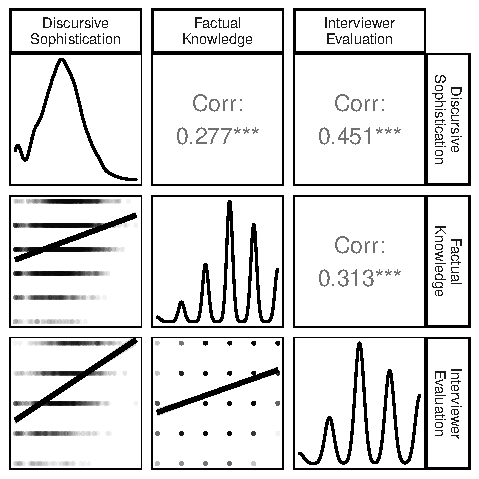
\includegraphics[height=.85\textheight]{../fig/anes2012_corplot.pdf}}
  \end{figure}
\end{frame}
% Now we want to look at desireable characteristics that should be associated with political sophistication -> political engagement as one standard validation check

\section{Additional Results}

\subsection{Topic Proportions -- 2012 \& 2016 ANES}
\begin{frame}{Topic Proportions -- 2012 \& 2016 ANES}\label{stm}
\begin{figure}
	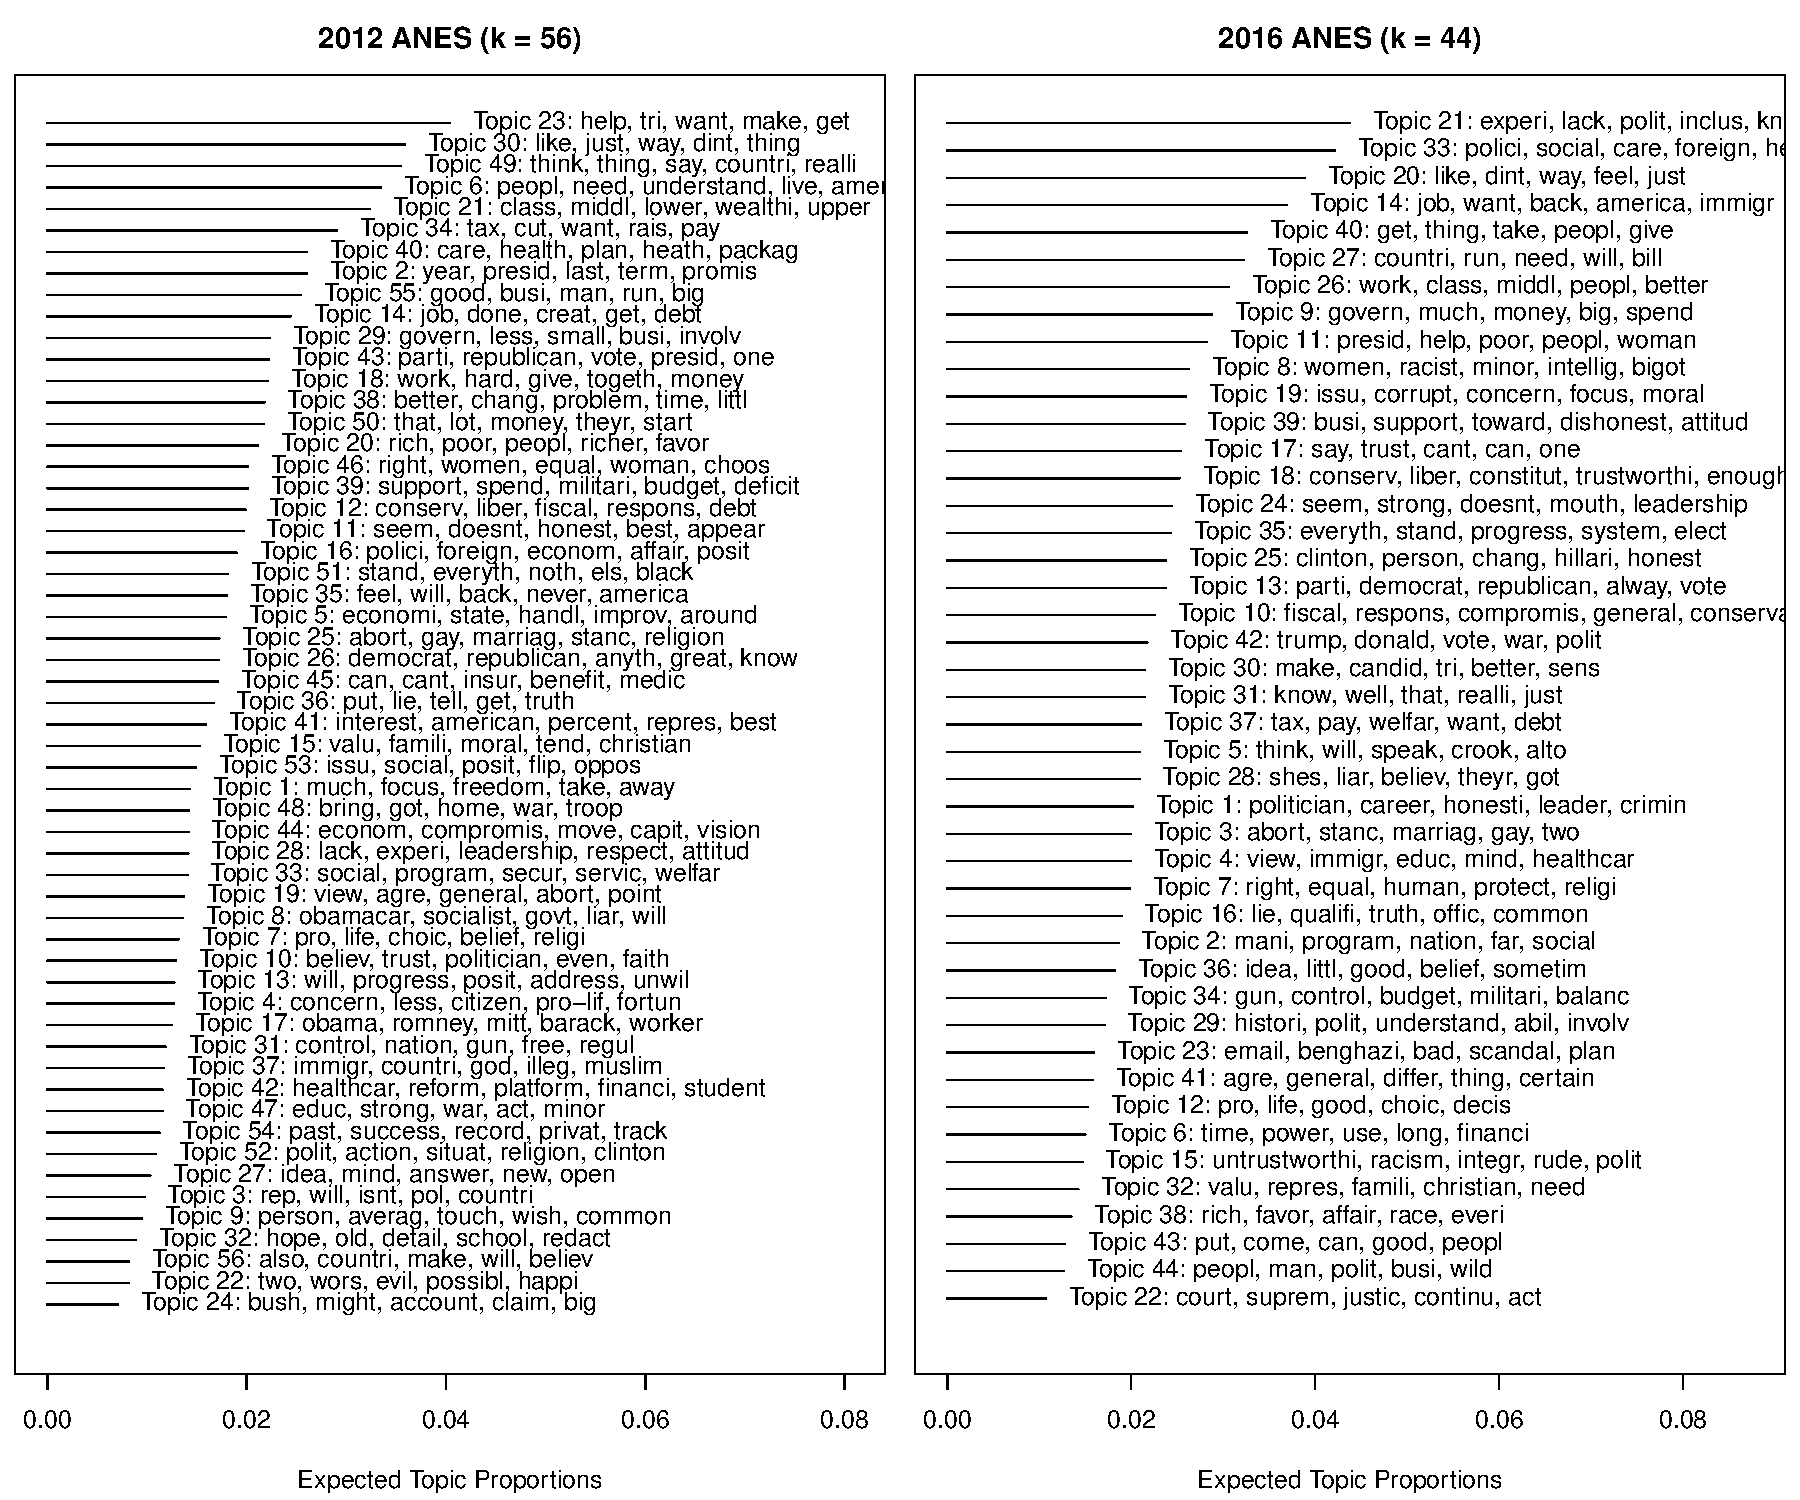
\includegraphics[height=.9\textheight]{../fig/anes_stm_prop.pdf}
\end{figure}
\end{frame}

\subsection{2008--2012 Swiss Referendum Survey}
% Here, we will look at political sophistication and competence
% Manual coding would be the ideal, Colombo as the gold standard

\begin{frame} %[allowframebreaks]
\frametitle{Comparison with Manually Coded Levels of Justification}
\emph{Data source}: 2008--2012 Swiss Referendum Survey, N = 26,621 (phone)
\begin{figure}
	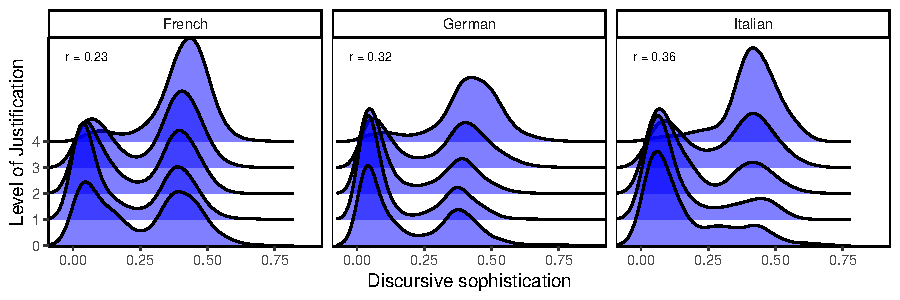
\includegraphics[width=\textwidth]{../fig/swiss_ggridges.pdf}
\end{figure}
\end{frame}
%Non-response: 4,917
% Manually coding would be the gold standard... How would it compare across 3 different languages -> very hard test!!!

\subsection{2015 YouGov Study}
% Here, we will look at political sophistication and competence
% Introduce the main point here!!

\begin{frame} %[allowframebreaks]
\frametitle{\hyperlink{retrieval_joint}{Accurate Information Retrieval}}\label{retrieval}
\emph{Data source}: 2015 YouGov Study, N = 1000 (online)
\begin{figure}
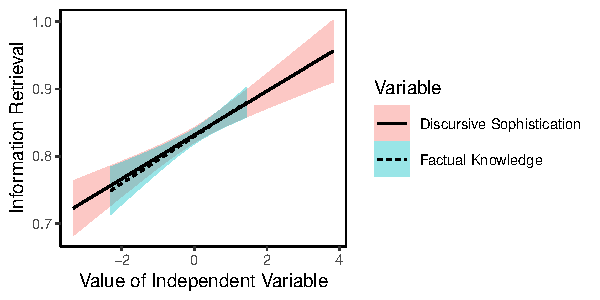
\includegraphics{../fig/yg_disease.pdf}
\end{figure}
\end{frame}
%Non-response: 48


\section{Robustness Checks}

%\subsection{Choosing the Number of Topics}
%\begin{frame}{Choosing the Number of Topics (2012 ANES)}\label{ktopics}
%  \begin{figure}
%  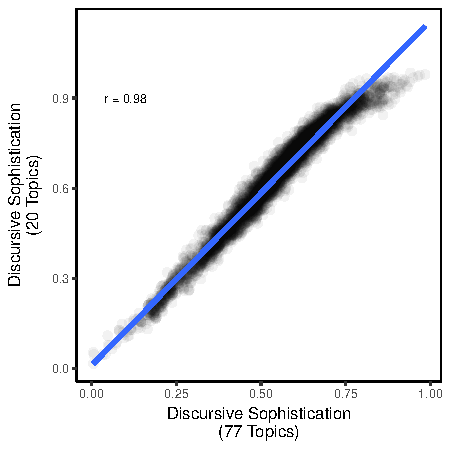
\includegraphics{fig/ktopic.pdf}
%  \end{figure}
%\end{frame}

\subsection{Control for Word Count}
\begin{frame}{\hyperlink{engagement}{Engagement and Participation -- Control for Word Count}}\label{engagement_lwc}
  \begin{figure}
  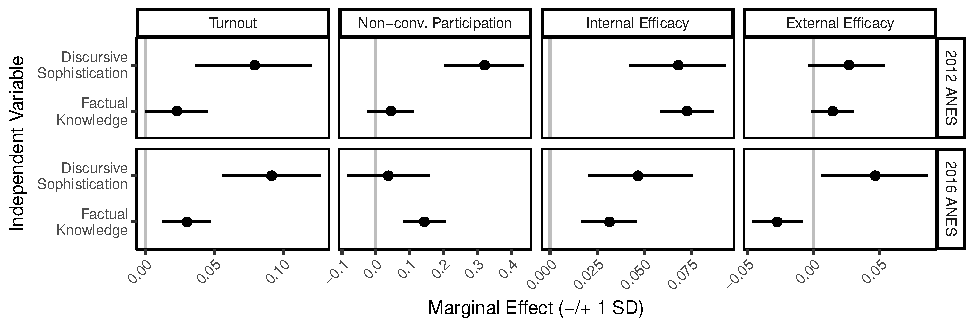
\includegraphics[width=\textwidth]{../fig/knoweff_lwc.pdf}
  \end{figure}
\end{frame}

\subsection{Control for Personality}
\begin{frame}{\hyperlink{engagement}{Engagement and Participation -- Control for Personality}}\label{engagement_personality}
  \begin{figure}
  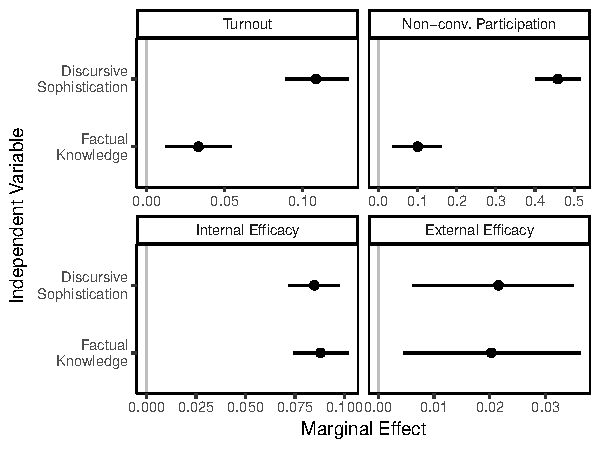
\includegraphics[width=\textwidth]{../fig/knoweff_personality.pdf}
  \end{figure}
\end{frame}

\subsection{Determinants of Sophistication}
\begin{frame}{Determinants of Sophistication}
\begin{figure}
	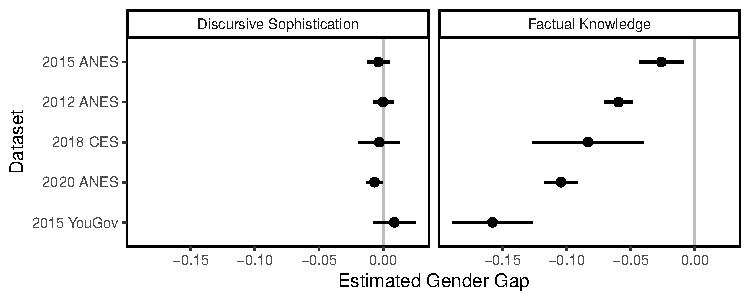
\includegraphics[height=.9\textheight]{../fig/determinants.pdf}
\end{figure}
\end{frame}

%\section{Additional Analyses}
%
%\subsection{Precision in Perceived Ideological Position}
%\begin{frame}{Precision in Perceived Ideological Position (2012 ANES)}\label{hetreg}
%  \begin{figure}
%  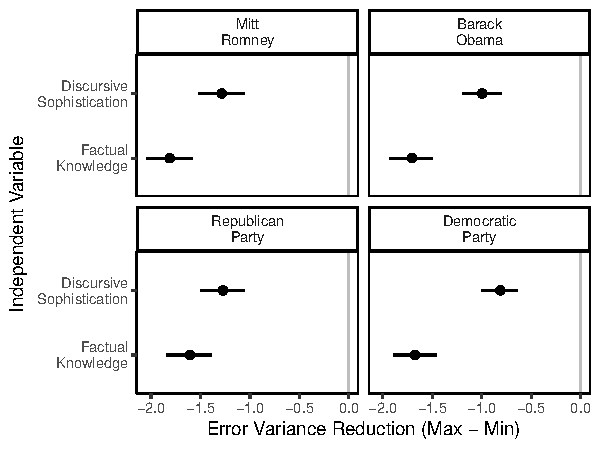
\includegraphics{fig/hetreg_pres.pdf}
%  \end{figure}
%\end{frame}
%
%\subsection{Consistency with Initial Vote Intention}
%\begin{frame}{Consistency with Initial Vote Intention (2012 ANES)}\label{prepost}
%  \begin{figure}
%  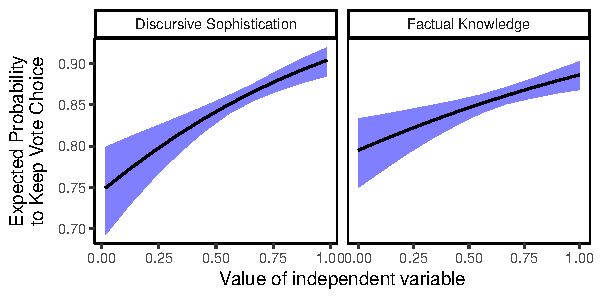
\includegraphics{fig/prepost_exp.pdf}
%  \end{figure}
%\end{frame}
%
%\subsection{Issue-Consistency: Support for Redistribution}
%\begin{frame}{Issue-Consistency: Support for Redistribution (2012 ANES)}\label{redistribution}
%  \begin{figure}
%  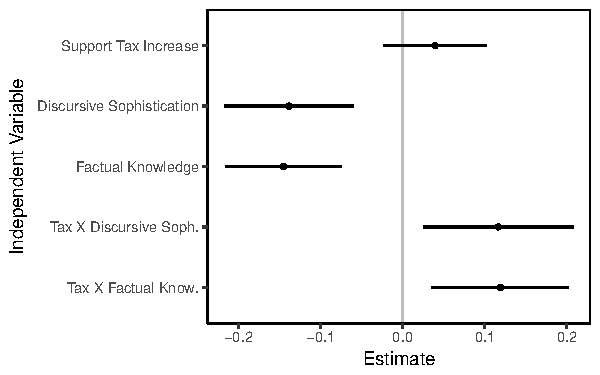
\includegraphics{fig/redistribution.pdf}
%  \end{figure}
%\end{frame}
%% Prior (2014): Visual Political Knowledge